\documentclass[10pt,twocolumn]{confpaper}

%%%%%%%%%%%%%%%%%%%%  INCLUDES  %%%%%%%%%%%%%%%%%%%%%%%%%%

\definecolor{darkgreen}{rgb}{0.0, 0.65, 0.0}

\ifthenelse{\equal{\COMMENTS}{yes}}{%
\newcommand{\mcnote}[1]{\textit{\textcolor{blue}{[marco]: #1}}} % Marco's comments
\newcommand{\lv}[1]{\textcolor{red}{(\textit{\textcolor{red}{LV:#1}} )}}
\newcommand{\rmnote}[1]{\textit{\textcolor{darkgreen}{[robert]: #1}}} % Robert's comments
\newcommand{\rbnote}[1]{\textit{\textcolor{orange}{[rudy]: #1}}} % Rudy's comments
\newcommand{\nf}[1]{\textcolor{red}{(\textit{\textcolor{red}{NF: #1}} )}}
}{
\newcommand{\mcnote}[1]{}
\newcommand{\lv}[1]{}
\newcommand{\rmnote}[1]{}
\newcommand{\rbnote}[1]{}
\newcommand{\nf}[1]{}
}


\newcommand{\supsym}[1]{\raisebox{4pt}{{\footnotesize #1}}}
\newcommand{\et}{\supsym{$\dag$}}
\newcommand{\ucl}{\supsym{$\diamond$}}
\newcommand{\ptn}{\supsym{$\star$}}
\newcommand{\ceq}{\supsym{$\ddag$}}


\usepackage{listing}
\usepackage[]{algorithm2e}

\renewcommand{\baselinestretch}{1.005} 


\definecolor{steel_blue}{RGB}{70, 130, 180}

\lstset{
basicstyle=\footnotesize\ttfamily\small,
frame=none,
language=Python,
numbers=none,
breaklines=true,
xleftmargin=0pt
}


\lstdefinelanguage{Pyretic}
{keywords={>>, >+, +, &, push, if_, elif_, else, pop, match, fwd, modify, set, mod, drop, $\triangleleft$, announce, withdraw}, 
  sensitive=true, alsoletter={-,>>,+,&,|,_},comment=[l][\footnotesize\sffamily\textbf]{\!}
}

\lstset{emph={View1, CA, CA-IN, as-path, med, no-prepend},
  keywordstyle=\color{steel_blue}\textbf}
\lstset{language=Pyretic}


%%%%%%%%%%%%%%%%%%%%  LOCALS  %%%%%%%%%%%%%%%%%%%%%%%%%%%%

\newcommand{\system}{iSDX\xspace}

%%%%%%%%%%%%%%%%%%%%  TITLE/AUTHORS  %%%%%%%%%%%%%%%%%%%%%


\date{}
\title{
{Concise Encoding and Querying of Sequences in Packet Headers}}
\author{
{Robert MacDavid\ptn, R\"udiger Birkner\et,} 
{Jennifer Rexford\ptn, Nick Feamster\ptn}\\
\ptn\normalsize{Princeton University}~~~\et\normalsize{ETH Z\"{u}rich}\\
}

%%%%%%%%%%%%%%%%%%%%  START OF DOCUMENT  %%%%%%%%%%%%%%%%%

\begin{document}
\maketitle
\thispagestyle{empty}

%\AcmCopyright
%\ToAppear

%\begin{sloppypar}

\abstract{
Network devices such as routers, switches, and firewalls forward traffic based on entries in their local forwarding tables. Although these forwarding tables conventionally make decisions based on a packet header field such as a destination address, attaching sets of attributes to flows during classification and making forwarding decisions based on attributes in that set can enable richer network policies. For example, devices at the edge of a network could add a tag to each packet that encodes a set of middleboxes to traverse, a set of egress locations, or a set of anycast destinations; simpler devices in the core of the network could then forward packets based on this tag. 

Unfortunately, naive construction of these tags can create forwarding tables that grow quadratically with the number of elements in the set or sequence--prohibitive for commodity network devices. In this paper, we present a compression algorithm that makes such encodings practical. The compression algorithm encodes sequences or sets (e.g., middlebox service chains, lists of next-hop network devices) in a compact tag that fits in a small packet header field. Our evaluation shows that the compression technique can encode common forwarding sequences for large networks using only a few bits and that the number of forwarding rules grows linearly with the number of elements in the set or sequence.
}



\ifthenelse{\equal{\onlyAbstract}{no}}{% !onlyAbstract



\section{Introduction}
\label{sec:intro}
%%%
%%% Forwarding Equivalence Class
%%%
Routing is increasingly more sophisticated than simply directing all traffic along a shortest path to the destination.  Depending on their header fields, packets may traverse a sequence of middleboxes, be subject to access-control policies, be multicast to a set of receivers, or be anycast to one of several equivalent servers.  Customizing the handling of the packets can require network switches to have a large number of forwarding rules that match on multiple header fields.  Fortunately, many packets are treated the same way.  Traffic flows that are treated identically by the network can be grouped into a single \emph{forwarding equivalence class} (FEC). If the edge of the network classifies each packet and tags it with a FEC, the interior switches can simply forward packets based on the tag, leading to substantial reductions in forwarding state.

%%%
%%% FEC is an index
%%%
The simplest and most common form of FEC tag is a flat tag, or \emph{index}. Historically, virtual circuit switching techniques like MPLS [cite MPLS] and VLAN [cite VLAN] follow this approach, and it is common in newer works as well~\cite{flowtags, sdx}.  Using the tag as an index worked well with traditional switches that support exact matches on a single header field, such as an MPLS label, VLAN tag, or destination MAC address.  However, index tagging solutions face three scalability challenges.  First, the size of the tag limits the number of FECs (e.g., the 12-bit VLAN tag can represent at most 4096 FECs).  Second, the number of FECs traversing a switch determines the number of forwarding rules and the churn that occurs after network events like link failures. And third, index tags offer no way to easily decode attributes associated with a FEC using a small amount of switch memory. 
%If a network node wishes to decode whether attribute $A$ is associated with a packet, it must determine whether the packet belongs to any FEC which is associated with $A$. If $A$ is associated with $N$ FECs, each of which has its own index, the switch requires $N$ rules for decoding $A$. 

%%%
%%% Matching on sequences
%%%
Fundamentally, the issue is that each FEC represents a \emph{collection} of attributes, yet two FECs that differ by only one attribute receive arbitrary indices. For middlebox steering policies, the FEC represents a sequence of middleboxes, and two FECs may differ in a single hop.  If the tag could represent a list of middleboxes efficiently, then switch $B$ in the example above would need just \emph{one} rule to differentiate between packets going to $C$ and $D$.
%%%
%%% Capabilities of newer switches 
%%%
Recently, commodity switches have emerged with more sophisticated capabilities.  OpenFlow 1.3~\cite{of13} supports \emph{wildcard} matching on multiple header fields. Emerging protocol-independent switches (programmable using languages like P4~\cite{P4}) support arbitrary headers that can be read, written, and matched in flexible ways.  These advances enable much more flexible ways to tag and match packets, beyond simple index tagging. 

%In the case of virtual circuit switching, the number of possible circuits can be exponential in the size of the network. Switches need to be programmed to react to every tag they may see, resulting in exponential memory usage. It may be the case that the majority of equivalence classes that a switch sees take identical egress ports, yet traditional tagging is unable to take advantage of this redundancy. Fundamentally, an equivalence class can be characterized by a set of attributes where that set is unique to that class. If two circuits differ by only a single hop, their attribute sets are unique and they are assigned different tags. Traditional solutions make no attempt to convey the similarity of the two sets in the tags, which could allow switches to be programmed with a single rule that reacts to both tags. We refer to these solutions as \textit{flat tagging} solutions. 


%Paragraph 3: "In this paper, we show that ...". This is the key paragraph in the intro - you summarize, in one paragraph, what are the main contributions of your paper given the context you have established in paragraphs 1 and 2. What is the general approach taken? Why are the specific results significant? This paragraph must be really really good. If you can't "sell" your work at a high level in a paragraph in the intro, then you are in trouble. As a reader or reviewer, this is the paragraph that I always look for, and read very carefully.

In this paper, we show how the set of attributes that define an equivalence class can be embedded in the assigned tag. The attributes of any tag can then be individually read using a small set of wildcard rules.  Such \emph{attribute-carrying tags} are much more compact, and lead to much smaller rule tables, than index tagging solutions.  We present efficient algorithms for generating compact tags that represent either \emph{sets} or \emph{sequences} of attributes.  We show how these tags can be used in several real applications, including our SDN-based Internet exchange point~\cite{isdx}.  Additionally, we show how these tags not only improve the scalability of existing systems, but also open new applications. We have made public the code library for incorporating our tagging scheme into any application. We perform evaluations on both real and synthetic datasets for our proposed applications and show that it can reduce the amount of switch memory by X. 

%Paragraph 4: At a high level what are the differences in what you are doing, and what others have done? Keep this at a high level, you can refer to a future section where specific details and differences will be given. But it is important for the reader to know at a high level, what is new about this work compared to other work in the area.

%Paragraph 5: "The remainder of this paper is structured as follows..." Give the reader a roadmap for the rest of the paper. Avoid redundant phrasing, "In Section 2, In section 3, ... In Section 4, ... " etc.

The remainder of this paper is structured as follows. In \S \ref{sec:background}, we give some area background and a few motivating applications. In \S \ref{sec:base_encoding}, we outline the basic ideas of our encoding scheme for attaching sets of attributes to packet headers. In \S \ref{sec:identifiers}, we improve the space usage of the base encoding. In \S \ref{sec:ordering}, we extend our encoding to support ordered sequences of attributes. In \S \ref{sec:evaluation}, we evaluate the encoding over both real and synthetic data sets. We discuss related works in \S \ref{sec:related}. The paper concludes with \S \ref{sec:conclusion}.






%\subsection{Common Ground}
%
%Although a diverse set of applications, each of these problems fits a common framework. As a packet enters a local area network, it is classified as belonging to some category of traffic. Associated with this category of traffic is a sequence or set. During classification, this sequence is somehow attached to the packet header.
%All three of these examples have a common framework: Packets are fit into categories as they enter a local area network, and associated with each category is some sequence of information. These sequences can be middleboxes, hosts, next-hop switches, or something else entirely. The sequence could be ordered, as in the case of middlebox paths, or unordered as in the case of feasible next-hops. In each case, the sequence is read by the local network switches to determine which direction to route the traffic. We refer to this reading of information as \textit{membership testing}, because routing choices are decided based upon which hosts or middleboxes are members of the sequence. 

%\subsection{Forwarding Table Matching On Tags}
%
%
%For this scheme of attaching information sets to packets to be feasible with commodity switches, it must be possible for membership testing to be implemented in the forwarding tables of switches. In switch TCAM tables, rules are are comparisons between a fixed string and the packet header, where the fixed strings are over the alphabet $\{0,1,*\}$. $0$ and $1$ are specific bit values, and $*$ denotes "don't care". We say that a packet header matches a string if for every bit in the header, either the bits are equal or one is a wildcard. Example usages include exact matches (strings with no wildcards), prefix matches (strings that end in wildcards), and reading of individual bits (strings with only one non-wildcard). 
%
%Various applications benefit from the use of TCAM 
%
% (TODO: cite some tagging works like flowtags and the original SDX?) have solved the problem of associating packets with information sets by generating a tag for each unique information set and repurposing one of the fields in the header for the tag. In the FlowTags work, each middlebox path had its own set of tags, which could fit into the IP Fragment Identification field. To determine if middlebox $X$ is the next-hop, switches must compare the tag to every tag which has $X$ as a next-hop using TCAM exact matches. This can result in a TCAM entry count exponential in the number of bits in a tag. In the SDX work, each set of next-hops had a unique tag which was placed in the destination mac field. Again, to determine if next-hop $X$ is correct, the tag must be compared against every tag which contains $X$ using exact TCAM matches. 
%
%In both works, the number of bits required can be quite small, but membership tests are expensive, requiring rules exponential in the tag size. TCAM is a very limited resource, and it would be desirable to design tags with the goal of decreasing the number of entries required for membership testing. 
%
%To combat these issues, we present a compression scheme which allows
%the encoding of sequences over a large number of elements, such as service chains or lists of BGP next-hops, into a format easily queried by commodity switches. We show how, with an additional algorithm, this scheme can be used to compress both ordered and unordered sets. Finally, we evaluate our algorithms across both synthetic and real datasets, and show not only does the number of bits needed by our compression scheme compete with the number of bits needed by tags, but that that each core switch need only a constant number of entries per membership test, versus a linear number of entries for the case of flat tagging.





\section{Sequence Encoding}
We have mentioned that, for flat tags, the number of forwarding table entries required for a single membership test can be large. 
To understand the problem, let us consider a simple example for the case of attaching lists of anycast hosts to a packet. Say that there is a local area network with five hosts $H = \{h_1, h_2, h_3, h_4, h_5\}$, and each packet that arrives will be classified as anycasting to one of four possible host sets: $s_1 = \{h_1, h_2, h\}$, $s_2 = \{h_1, h_2, h_3\}$, $s_3 = \{h_1, h_3\}$, or $s_4 = \{h_3, h_4, h_5\}$. In a flat tagging solution to this problem, each unique set will be assigned a single tag, and thus a packet which can be forwarded to the $i$th set will receive the $i$th tag. Now, for an intermediate switch to determine, using exact tag matches, if a packet can be forwarded to host $h_1$, it must check whether the packet has been assigned to $s_1, s_2,$ or $s_3$. The number of entries required is proportional to the number of sets which contain $h_1$, in this case 3. In the worst case $h_1$ would be a member of almost every group, and testing for $h_1$ would required a number of checks linear in the number of tags. 


\subsection{Sequence Bitmasks}

For the sake of explanation, assume that it is possible to attach an arbitrary
amount of metadata to each packet the moment it is classified,
and that forwarding table entries are
able to read and write to this metadata arbitrarily. We can easily use this hypothetical
metadata to test for membership of any sequence element. If there are $N$ possible elements that appear in any sequence, we can write $N$ bits to the
metadata: the $i$th bit corresponds to the $i$th element. The moment the packet is classified, the $i$th bit is set to 1 if the $i$th element is present in the sequence for that class of packet, and 0 if it is not. As a result, if we wish to test for membership of element $e$, we need only check that $e$'s bit is 1 in the metadata before rerouting, rather
than exact matching on every tag that contains $e$.

Of course, we cannot attach arbitrary metadata to packets. Rather, one common technique is to repurpose fields in the header for storing tags. In the FlowTags paper, the Fragment Identification field is used. In SDX, the destination MAC stores the tags. In both cases, there is a hard limit on the size of tags to at most a few bytes. The scheme of creating a bitmask to encode a set of elements will fail the moment the universe of elements grows too large. This further motivates our optimized encoding scheme.


\subsection{Multiple Masked Sets}

 As our scheme currently stands, we are assigning a single bit of the metadata bitmask to every
element in the universe of elements. If we have more elements than bits in the header field used for tagging, this approach immediately fails.

The purpose of the metadata bitmask attached to each packet is to concisely convey whether each element is contained in the set for that packet class or not. The bitmask can be thought of as recovering the desired list of elements by masking some \textit{superset} which contains all possible elements. 

\begin{figure}[t!] 
\begin{minipage}{1\linewidth}
\begin{subfigure}[b]{0.96\linewidth}
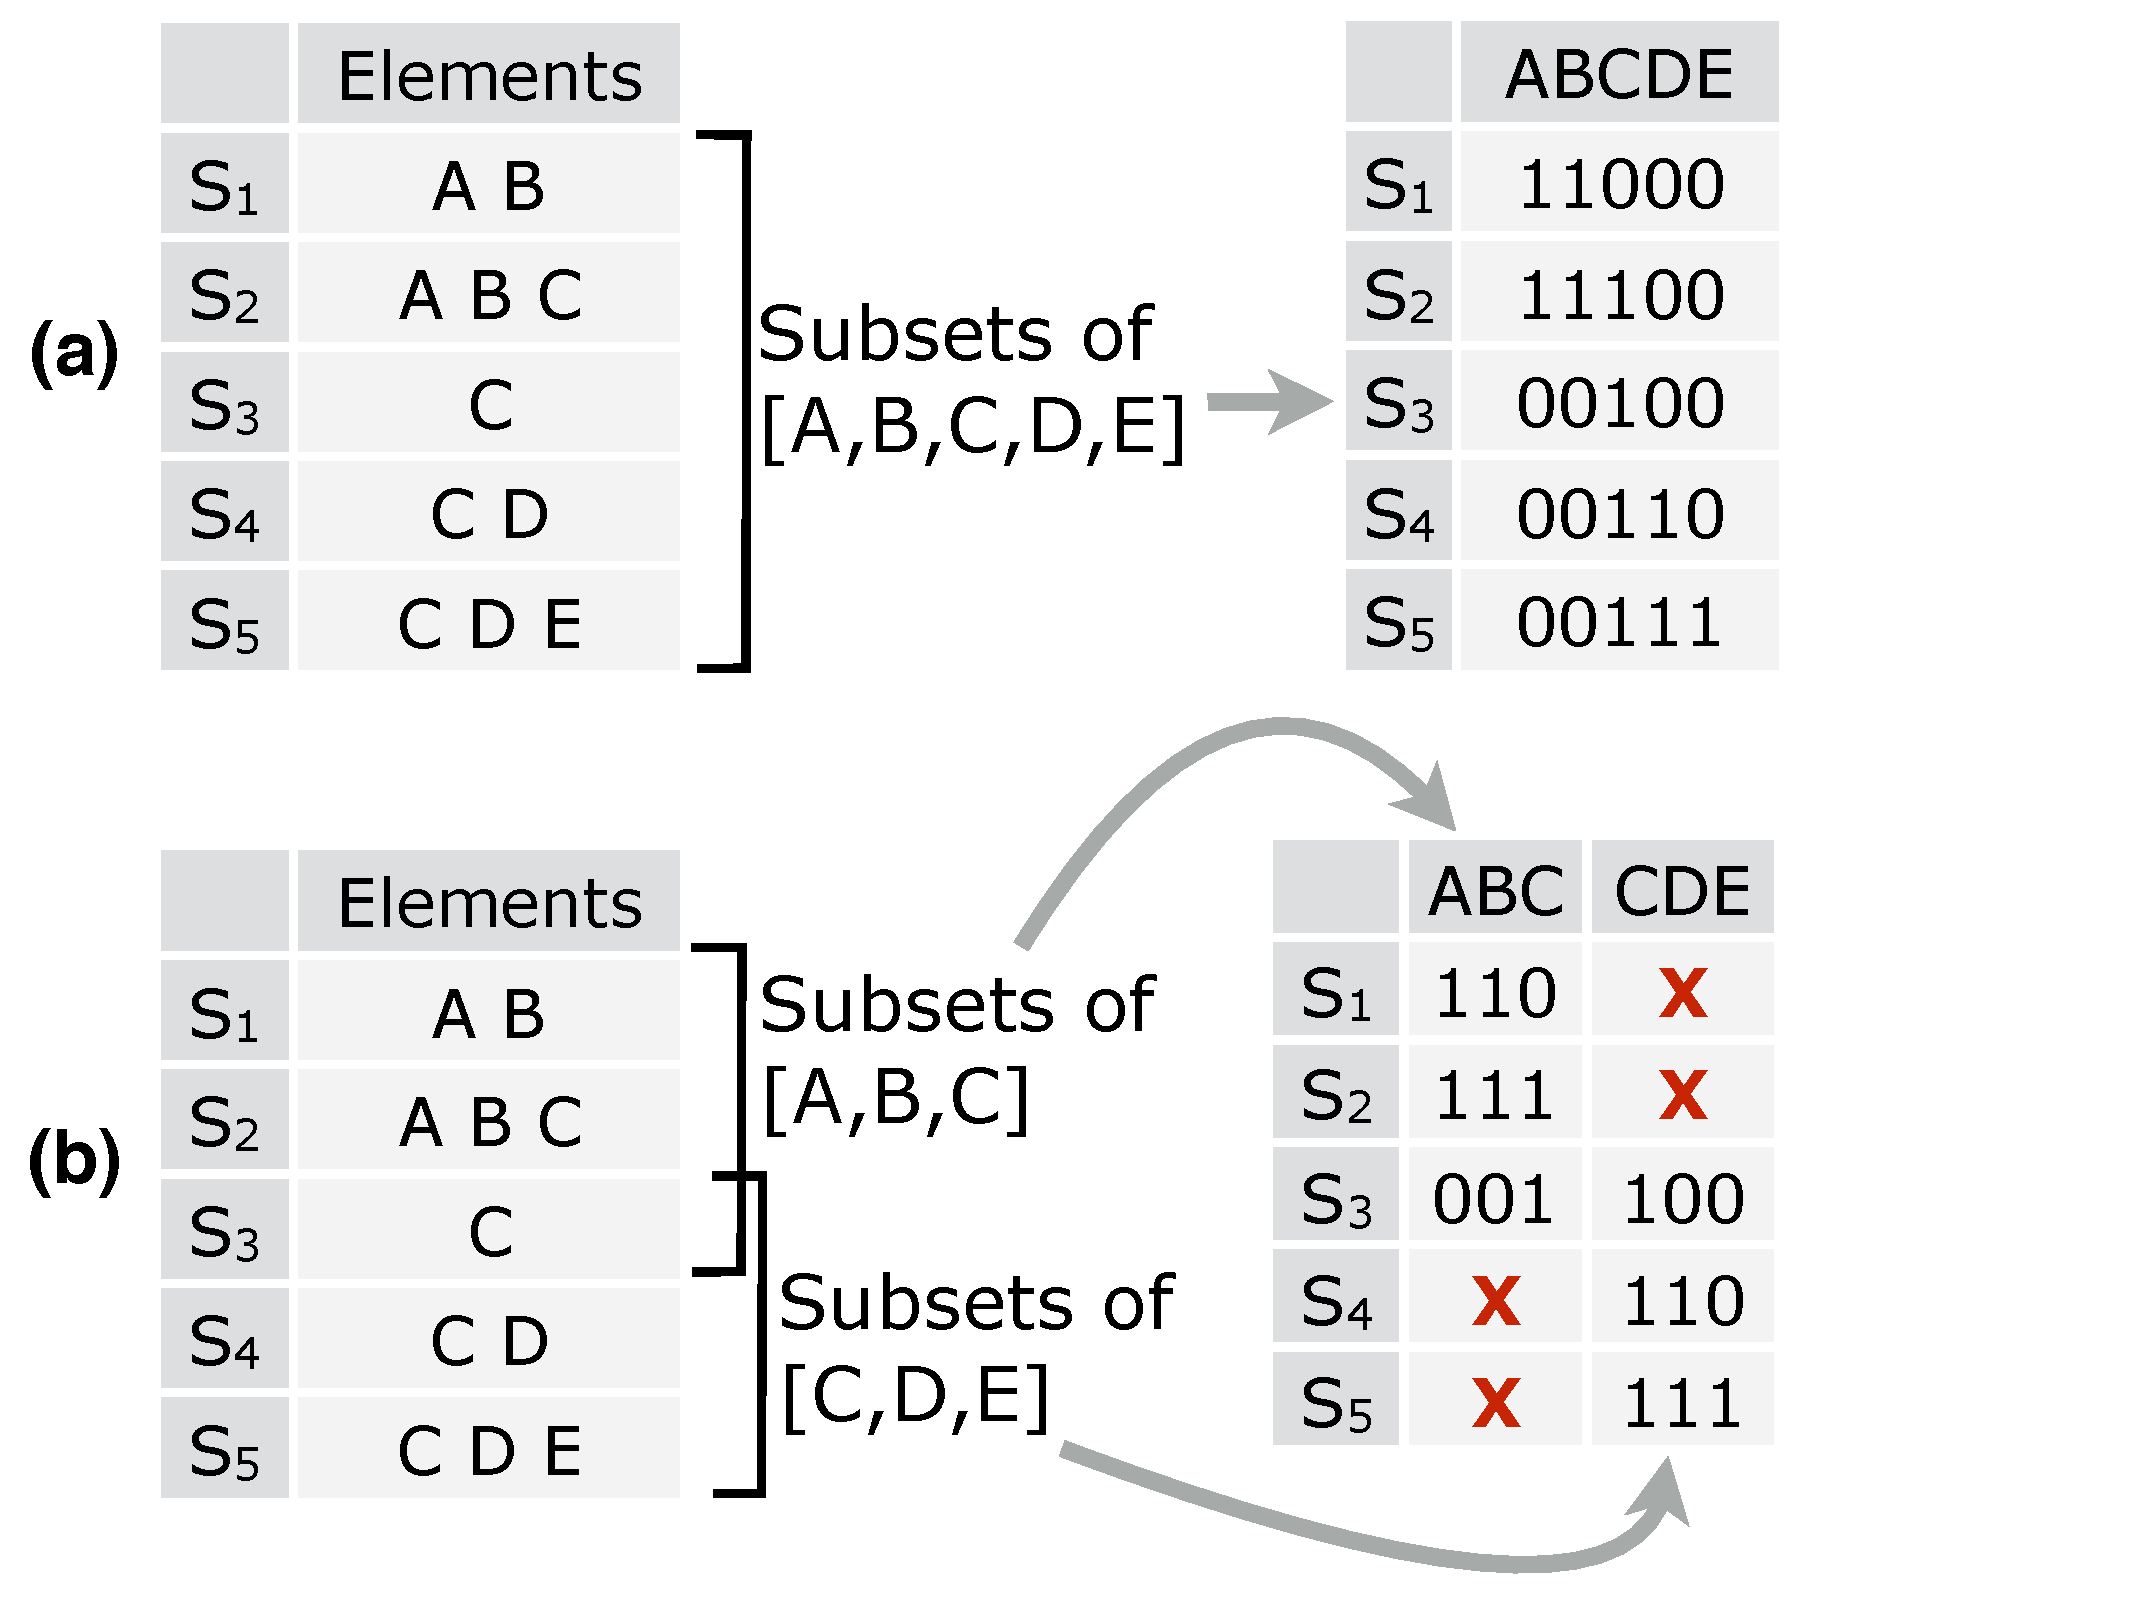
\includegraphics[trim={0 0 5.5cm 0}, clip, width=\linewidth]{figures/masking}
\end{subfigure} 
\begin{subfigure}[c]{0.96\linewidth}
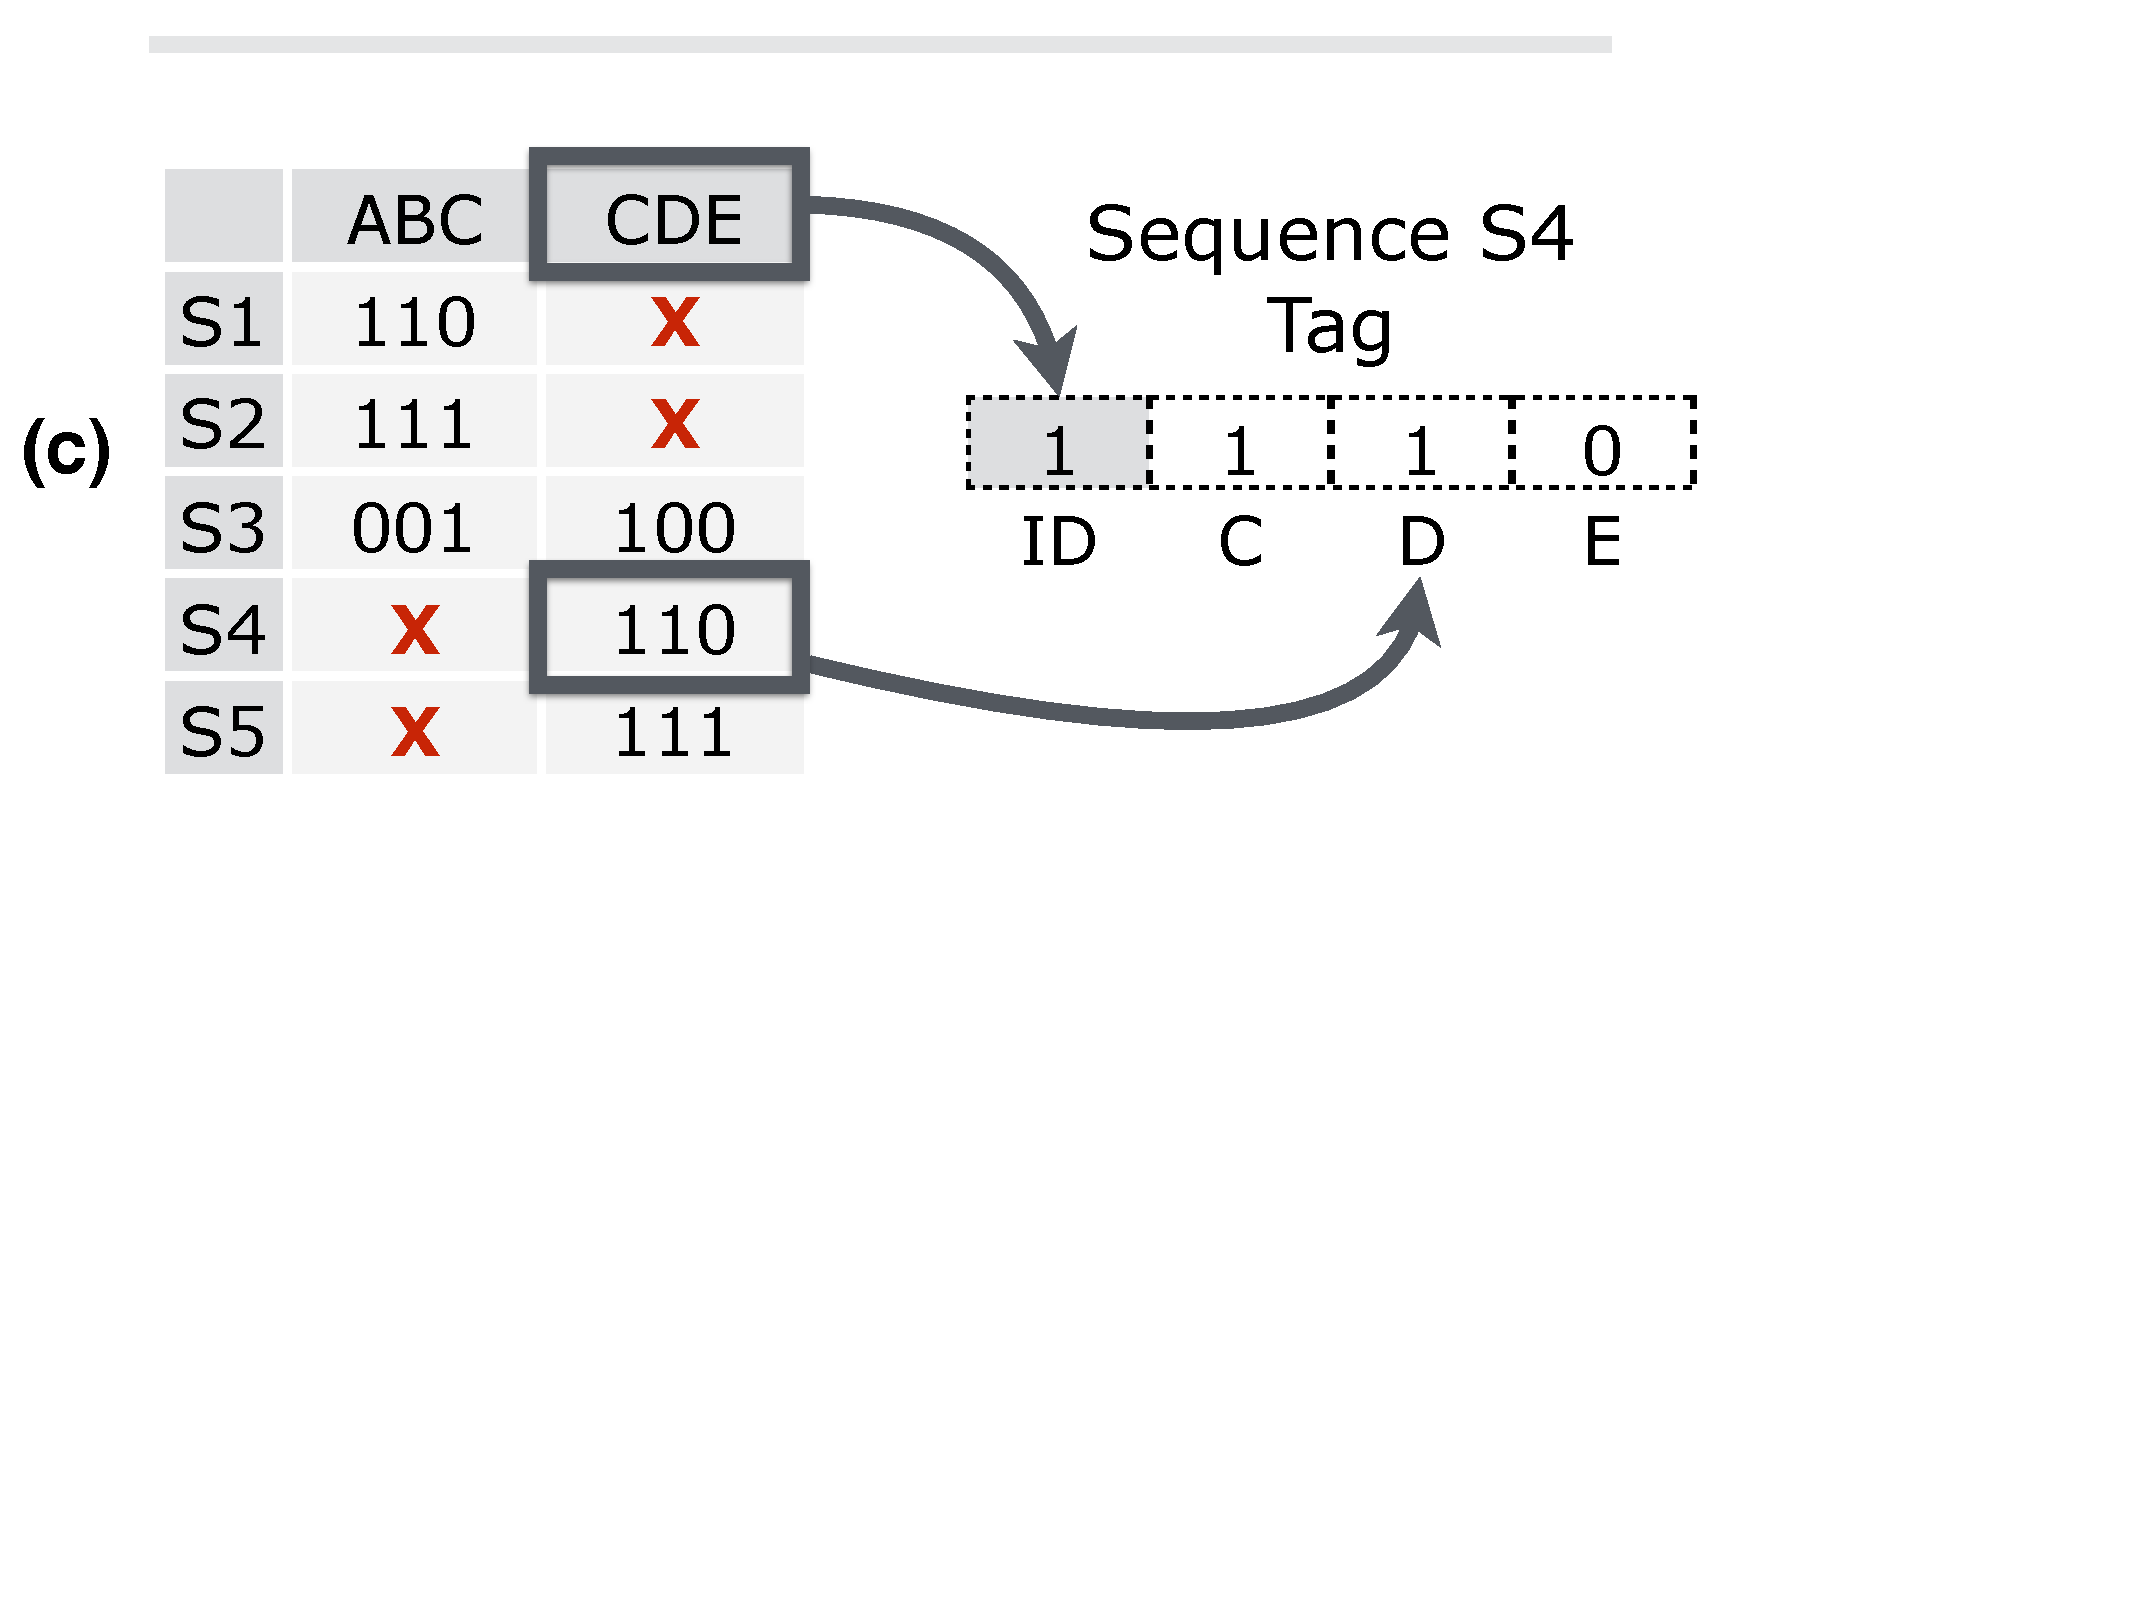
\includegraphics[trim={0 13cm 5.5cm 0}, clip, width=\linewidth]{figures/making_metadata}
\end{subfigure} 
\end{minipage} 
\caption{This figure demonstrates two different ways to recover sequences. In (a), the sequences are recovered by masking over $[A,B,C,D,E]$. In (b), the sequences are recovered by masking over either superset $[A,B,C]$ or set $[C,D,E]$. An X denotes that the sequence cannot be fully recovered by masking over the given set. (c) shows how, if each superset is identified by a binary integer, each sequence can be converted to a tag consisting of an identifier and a bitmask.}
\label{fig:masking}
\end{figure}

Consider the example in figure \ref{fig:masking}(a), where the left matrix contain the lists of elements that we wish to recover, and the right matrix shows the bitmasks we would currently generate. Figure \ref{fig:masking}(b) shows that the elements can be broken up into two categories: those which can be generated by masking over the superset $[A,B,C]$, and those which can be generated by masking over $[C,D,E]$. If we can add to our tag an identifier of the superset over which we are masking, we can have a reduced mask size! As shown in figure \ref{fig:masking}(c), if superset $[A,B,C]$ is identified as superset $0$, and $[C,D,E]$ is identified as superset $1$, then the tag for a packet class $p_4$ which is mapped to set $[C,D]$ becomes $1110$, which is shorter than simply masking over the complete universe.

Now, if a switch wishes to test for membership of element $D$, it must simultaneously check (1) the identifier for the superset that contains $D$ and (2) the bit in the bitmask which corresponds to $D$. Thus, the check that would be generated is\\
\noindent
{%\footnotesize
$\texttt{tag=1*1*} \rightarrow \texttt{action}(A)$\\
}
Where the first bit in the tag match is for the superset identifier, and the
remainder is for the mask.

However, looking again at figure \ref{fig:masking}(b), the case of testing for $C$'s membership is not so simple. Since $C$ appears in both supersets, we must check whether $C$'s bit is 1 in either superset mask. For example, if we had the rule\\
\noindent
{%\footnotesize
$\texttt{C in tag} \rightarrow \texttt{action}(A)$\\
}
This would be augmented under our scheme to become\\
\noindent
{%\footnotesize
$\texttt{metadata=0**1} \rightarrow \texttt{action}(A)$\\
$\texttt{metadata=11**} \rightarrow \texttt{action}(A)$\\
}
Therefore, depending upon the matrix construction, membership tests may still require multiple TCAM entries. If no superset is too large to fit into the mask, it is feasible to merge columns of the matrix to create new, larger supersets which can decrease the inflation factor. However, this can only be performed until the supersets of each column become too large to fit into the available bit space. For example, in figure \ref{fig:masking}(b), the two columns could be merged into $[A,B,C,D,E]$ to eliminate the inflation of $C$ rules. This would decrease the identifier size from 1 to 0 bits and increase the mask size from 3 to 5 bits. There is a 
balance to consider between the size of the superset identifier, the mask size, and the number of rules for membership testing, and when considered formally an optimization problem arises.




\section{The Formal Problem}
When constructing the supersets, there are two different objectives to keep in mind: minimizing the number of bits required by the superset identifier and mask, and minimizing the number of TCAM entries required for membership tests. If the goal was simply to minimize the number of bits required, we would have no bits for the mask and dedicate the entire tag to the identifier. This is flat tagging, and the number of TCAM entries required for membership tests would be maximized. If the number of bits for tagging was unconstrained, we would have no bits for superset identifier and simply have one large mask, causing each membership test to require only one TCAM entry. The problem only becomes interesting once both objectives are considered simultaneously, which we will now formalize. 

Let $P = \{p_1, p_2, \dots, p_N \}$ be the list of sets that will need to be recovered by header tags. The union of all these sets recovers the universe of all possible elements that we will see, $U =
\{1, 2, \dots, M\}$. Associated with
each element $j$ of the ground set $U$ is a weight term $w_j$. This weight term corresponds to the number of times the membership of $j$ is tested across the network. This will allow our algorithm to attempt to minimize the number of supersets that an element appears in if it needs to be tested for frequently. 

The goal of an algorithm which generates a superset encoding is to partition $P$ into $Z$ groups and union each group to create supersets $\{
s_1, s_2, \dots, s_Z \} = S$ such that the following function is minimized:

\begin{samepage}
$$ \min \sum_{j \in U} w_j \cdot a_j $$

Subject to

$$ \log_2{Z} + \max_{s_i \in S}\{s_i\} \le B $$

\end{samepage}

Where $a_j$ is the number of supersets that element $j \in U$ belongs to, and $B$ is the maximum number of bits that our tag can use. The objective function reflects the number of TCAM entries required for all membership tests. If the network tests for the membership of element $j$ $w_j$ times, and $j$ appears in $a_j$ supersets, then our approach requires $a_j w_j$ TCAM entries. 
The constraint shows that a superset construction is feasible if the identifier size plus the mask size is less than the bit constraint $B$. The identifier size is $\log_2{Z}$ if $Z$ is the number of supersets, and the mask size required is the maximum superset size, or $\max_{s_i \in S}\{s_i\}$.

We suspect that this problem is NP-Complete for \mbox{$M > B$}, but a proof of the claim is left as future work. 

\subsection{A Greedy Algorithm}

Although the problem may be hard, we can still formulate heuristics for constructing good-enough solutions. We begin with $N$ supersets, where superset $i$ is the $i$th list wish wish to recover. This solution is, by construction, able to generate every required element list, but it may not be feasible. $N$ may be so large that the superset identifier will dominate the metadata and exceed the bit limit. This solution will also certainly require a large number of TCAM entries, as no sets have yet been combined into supersets.

In the first step of the algorithm, we delete any supersets which are subsets of other supersets. If superset $s_i$ is $[A,B,C]$, and superset $s_j$ is $[B,C]$, then there is no use for $s_j$ and it may be deleted. Deletion strictly improves the solution because any subset of $s_j$ can still be recovered from $s_i$, and the superset identifier decreases in size as the number of supersets decreases. In practice, this reduces the number of sets down from hundreds of thousands to less than one hundred.

In step two, we attempt to greedily decrease the number of bits required by our feasible solution by merging pairs of small supersets together that do not increase the maximum mask size when unioned. The idea is that this will decrease the number of sets and thus the size of the superset identifier will decrease. This step repeats until every feasible merging action would increase the number of bits required. 

In step three, we improve the remaining supersets in an iterative greedy fashion. We consider all feasible mergings of pairs of supersets, where a feasible merge is a union of the two supersets which does not result in the new mask size exceeding the bit limit. The \textit{benefit} of a merging is the decrease in the number of flow rules which will result
from the merge. The decrease is the sum of the weights of each participant which appears in the intersection of the two supersets, where the weight is the number of flow rules in which the participant appears. This is because after a merging of two sets, every participant which appeared in the intersection now appears one less time across the supersets, and thus every rule they appear in can be replicated one less time. 

With these definitions in mind, the full algorithm is as follows:

\begin{algorithm}
 \KwData{feasible supersets $S = \{s_1, s_2, \dots, s_M\}$}
 \KwResult{a list of supersets with maximally decreased rule inflation }
remove subsets from $S$\;
let $A =$ the set of merge pairs which don't increase bits required\;
\While{A is nonempty}{
  choose pair $(s_i, s_j) = a \in A$ with smallest union\;
  merge sets $s_i$ and $s_j$\;
  update $A$\;
 }
let $A =$ the set of feasible merge pairs\;
remove any subsets from
\While{A is nonempty}{
  choose $(s_i, s_j) = a \in A$ with greatest benefit\;
  merge sets $s_i$ and $s_j$\;
  update $A$\;
 }
\end{algorithm}

The loops consider all pairs of supersets in each iteration in the worst case, so they have a quadratic running time. Fortunately, the removal of subset supersets in the first step, which runs linearly on lists of supersets with high redundancy, reduces the number of supersets in such lists to a small constant, so the running time is reasonable.

\subsection{Handling Updates}

We have given an algorithm for computing a static solution, but not all applications will be static. For middleboxes, new paths can be introduced, and existing paths can be modified. For IXP case, routes are announced and withdrawn continuously, meaning the list of valid next-hops for many prefixes are constantly changing. Therefore, we must give a procedure for handling dynamic updates to the superset matrix.

We begin with a feasible solution as output by our algorithm, which is a collection of supersets and a mask for each element set. We consider both cases of a new set or a modified set identically. We first generate a new superset for the new/modified set. If this new superset is a subset of an existing superset, we remove it. 

Each time a prefix is announced or withdrawn by a participant, we consider that prefix's new list of valid next-hops. If it is still a subset of some superset, we need only update the mask. 

If the new set is not a subset of any superset, we attempt to merge the new superset with an existing superset via the same greedy procedure we applied to the static context. If no merging is possible, we leave it as its own superset. If the introduction of the new superset causes the bit limit to be exceeded, we recompute the static solution entirely as a worst-case scenario. In our evaluations, we have found the worst-case scenario is never needed.



\section{Encoding Attribute Sequences}
\label{sec:ordering}
In some applications, the \emph{order} of attributes is important.  For example, in service chaining, traffic must traverse middleboxes in a specified order.  In this section, we extend our scheme for encoding \emph{sets} of attributes to support \textit{sequences} of attributes.  We first propose a simple representation of the attribute sequences in a sequence graph.  Next, we discuss how to encode sequences when the attributes follow a partial order.  Then, we show how to encode sequences in general, even when the attributes do not form a partial order.

\subsection{Sequence Graph of Attribute Orderings}
When the tag must encode a sequence of attributes, we need an effective way to identify what \emph{ordering} of attributes can occur.  Figure~\ref{fig:ordering}(a) shows four equivalence classes ($S_1$-$S_4$) with different sequences of attributes ($A$-$F$); for example, $S_2$ has the attribute sequence $E$-$A$-$B$, whereas $S_4$ has $A$-$B$-$C$-$D$.  We can generate a \emph{sequence graph} where each node is an attribute, and a directed edge from node $u$ to node $v$ exists if $u$ appears just before $v$ in any of the sequences.  For example, the sequence graph in Figure~\ref{fig:ordering}(b) has an edge from $E$ to $A$ and from $A$ to $B$ because of $S_2$, and from $D$ to $F$ because of $S_3$.  Each sequence in the input data corresponds to a path through the sequence graph.  If the sequence graph is acyclic, the attributes form a partial order, making it easier to encode all of the the sequences concisely.

\begin{table}
    \begin{tabular}{| l | l | l |}
    \hline
    Attribute & Unordered Match & Ordered Match\\ \hline
    A & $1011**$ & $1011**$ \\ \hline
    B & $101*1*$ & $10101*$ \\ \hline
    C & $101**1$ & $101001$ \\
    \hline
    \end{tabular}
    \caption{Wildcard strings for ordered versus unordered attributes. %In the unordered case, the string matches if the target attribute bit is 1, and does not depend upon the bits of other attributes.
     In the ordered case, the string only matches if the target attribute bit is 1 and all bits for attributes preceding the target attribute are 0. This ensures only matching on the next attribute in the ordering succeeds.} 
    \label{tab:ordering}
\end{table}

\subsection{Sequences that Form a Partial Order}
If all of the attributes form a (partial) order, we can easily construct a single ordered list of all attributes where each input sequence is a subsequence. We refer to such a sequence as a \emph{supersequence}.  A supersequence can be computed by processing the nodes of the (acyclic) sequence graph in order. 
%
Then, sequences are selected, each as the union of some input sequences. A tag of a sequence would then include identifier together with a mask of its attributes based on the order of the supersequence.  Table \ref{tab:ordering} illustrates an example of wildcard rules imposing such an ordering for a sequence with attributes $A, B, C$ that was assigned the identifier $101$.  If the ordering dictates that an attribute $B$ must appear after $A$, then any wildcard rule for decoding $B$ must check that the $B$ bit is 1 and the $A$ bit is 0. This causes the wildcard rule to only successfully match if no other attributes that come before $B$ appear in the set. %In other words, testing for $X$ only returns true if tests for all attributes before $X$ returns false.

\subsection{Not-Aligned Ordering Constraints}
Sometimes, there does not exist a supersequence of attributes that all sequences follow its order. This is case  if for two attributes $B, A$,  $B$ appears before $A$ in some sequences, but $A$ appears before $B$ in others. Similarly, this happens when $B$ appear before $A$ in a sequence and $A$ has to appear before $B$ based on transitivity of other attributes. We refer to that as order-inconsistency.  In such cases the graph $G$ contains a cycle. We describe two approaches to deal with this scenario. 

\textbf{Approach I:} The first approach begins with the input sequences. In each step, pairs of supersets are considered as long as their merging does not result in order-inconsistency. A pair is selected based on similar criterions as for the non-ordered sets. Finally, for each superset in the result, an identifier is allocated based on a potential order of the corresponding attributes.

\textbf{Approach II:} The first approach can sometime result in a large number of sequences that cannot be further merged. The second approach is more flexible by allowing the merging of two sequences even if this results in order-inconsistency. We solve the inconsistency by finding a supersequence with multiple appearances of some of the attributes such that merged sequences can be described as subsequences. 

To do so systematically, we construct the sequence graph $G$, shown in \ref{fig:ordering}(b) for the sequences  in \ref{fig:ordering}(a). We then run an algorithm for finding Strongly Connected Components (SCCs) on this graph. A strongly connected component is a set of nodes such that for every pair of nodes $u$ and $v$ in the set, $u$ has a path to $v$ and vice versa. In this context, every SCC corresponds to a set of incomparable elements.  Figure \ref{fig:ordering}(d) and (e) shows the result of using this new ordering to modify each sequence.  
Figure \ref{fig:conflict_res} details the process for determining which elements to split to create a new, totally ordered universe.


\begin{figure}[t!] 
\begin{minipage}{1\linewidth}
\begin{subfigure}[c]{0.96\linewidth}
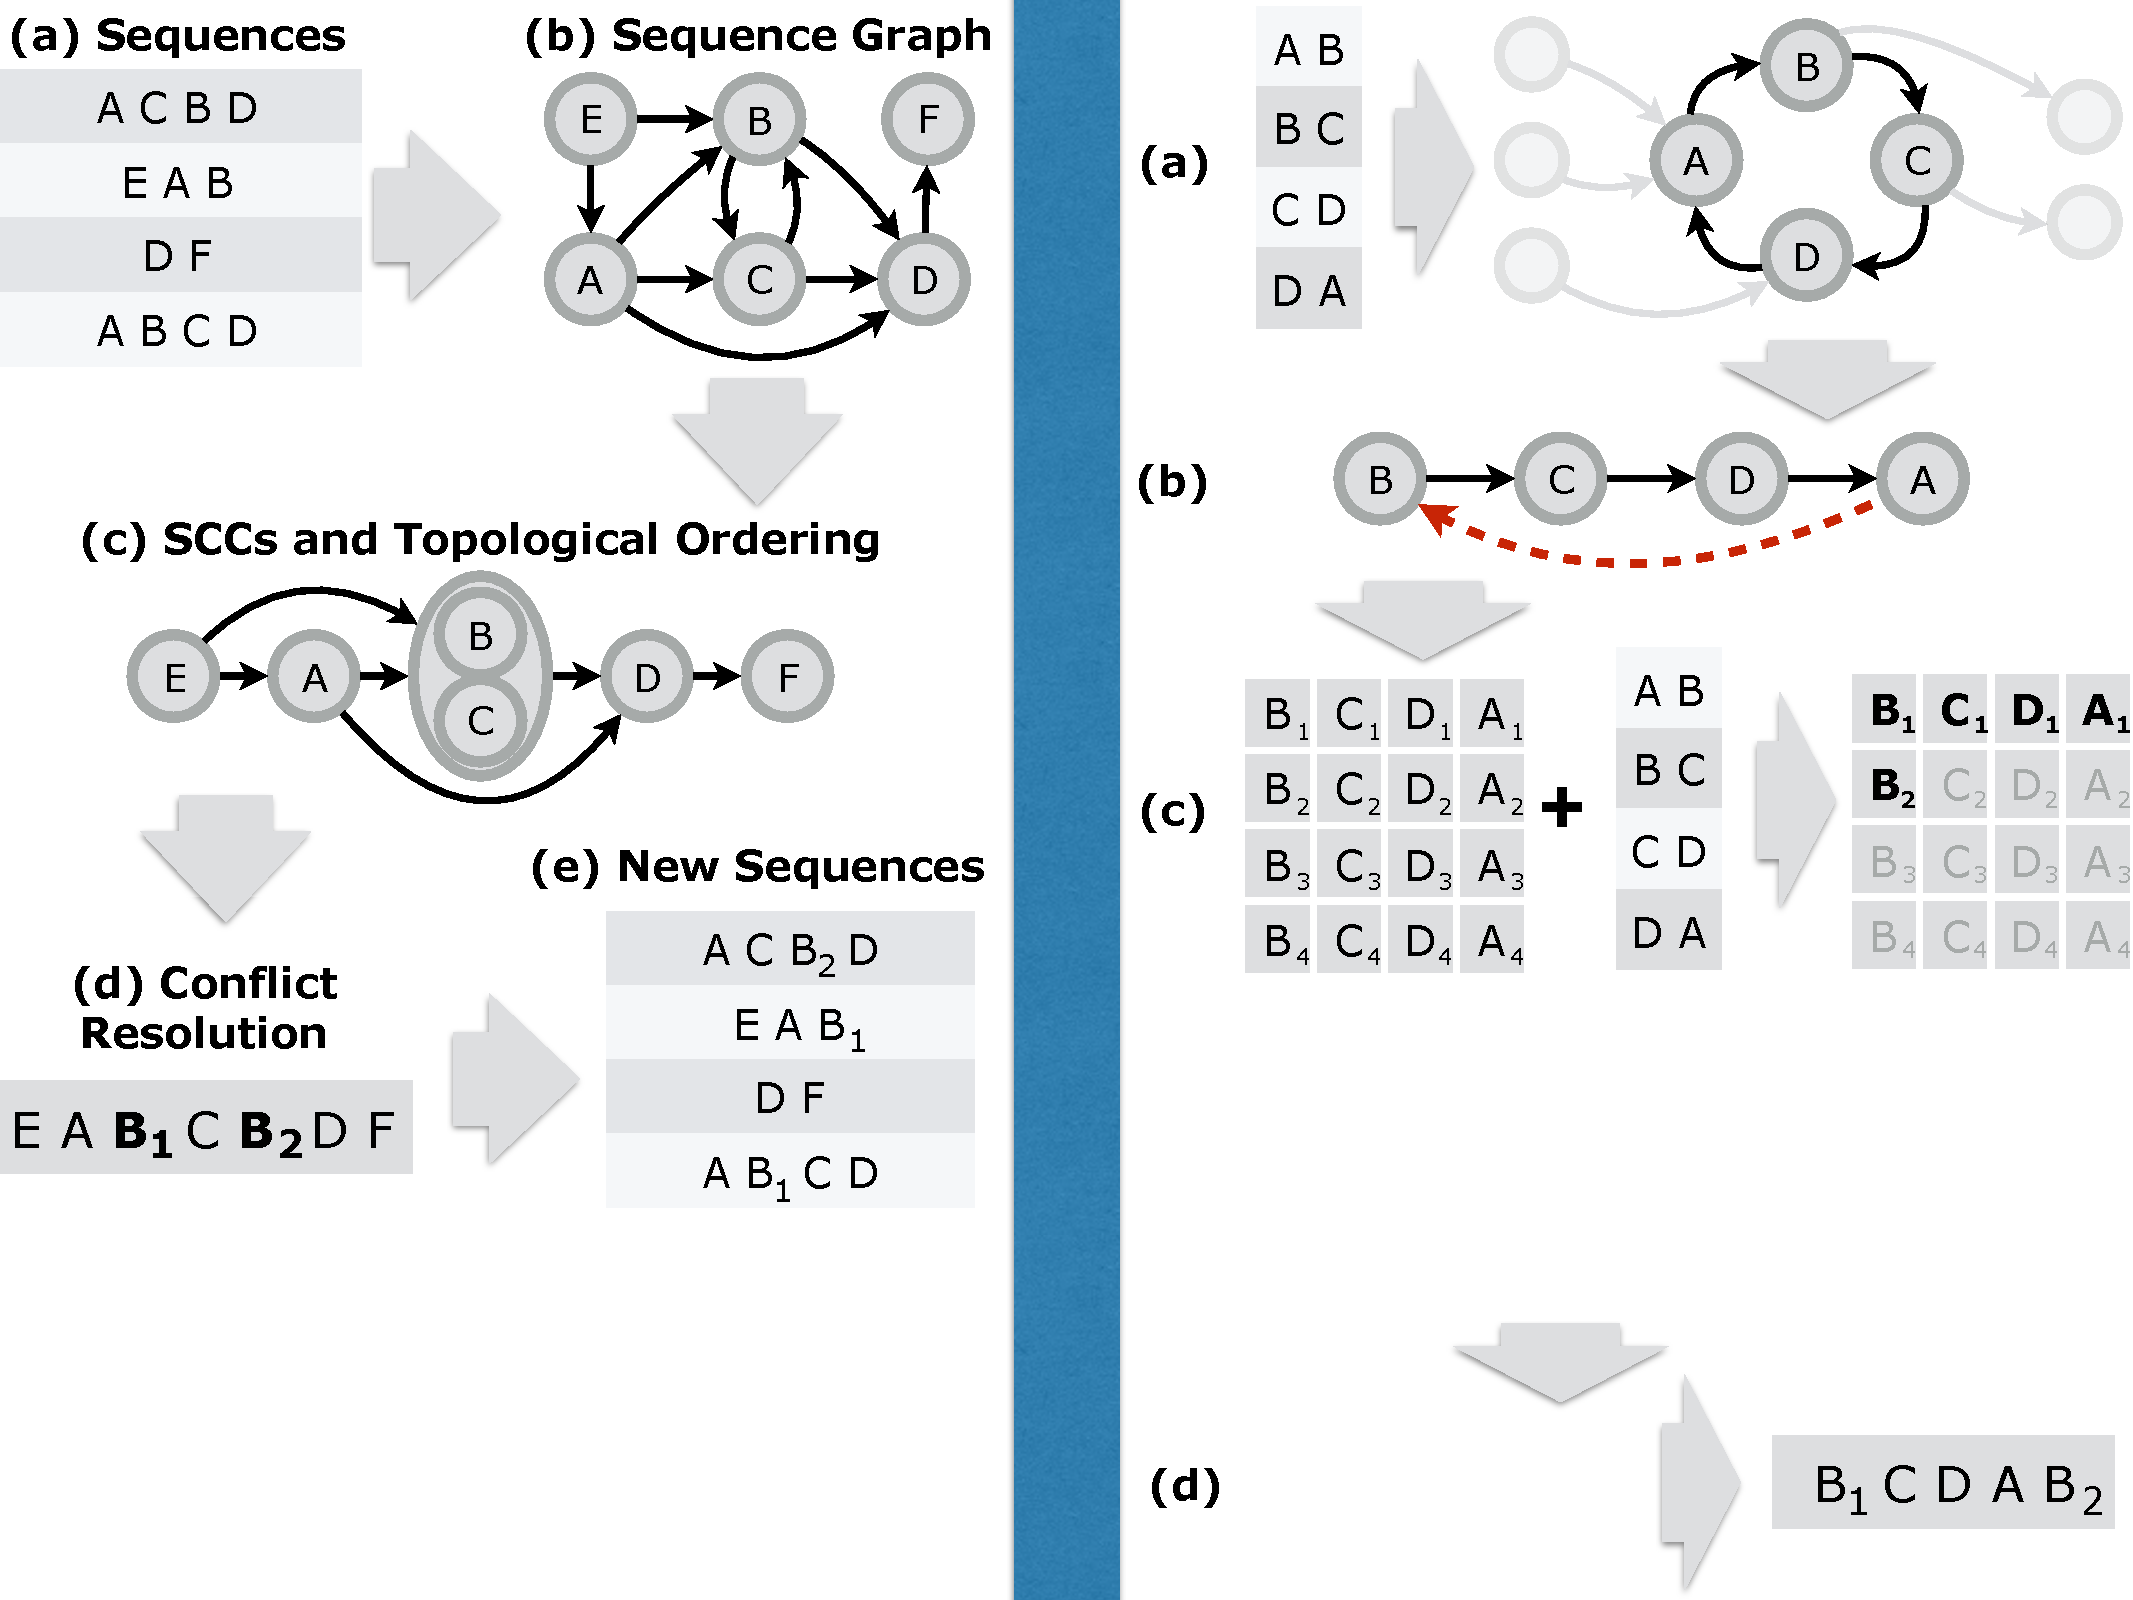
\includegraphics[trim={0 6cm 19.2cm 0}, clip, width=\linewidth]{figures/partial_ordering}
\end{subfigure} 
\end{minipage} 
\caption{Not-aligned ordering constraints. (a) shows the four input ordered sequences. In (b) illustrates the corresponding sequence graph $G$.. (b) shows the disjoints SCCs  (Strongly Connected Components) of $G$. Each SCC corresponds to a set of incomparable elements. (d) describes the result of splitting elements to resolve order-inconsistency, which is covered in more depth in figure \ref{fig:conflict_res}. In (e), the original sequences are modified with the splits such that each sequence adheres to the constructed ordering.}
\label{fig:ordering}
\end{figure}



\begin{figure}[t!] 
\begin{minipage}{1\linewidth}
\begin{subfigure}[c]{0.96\linewidth}
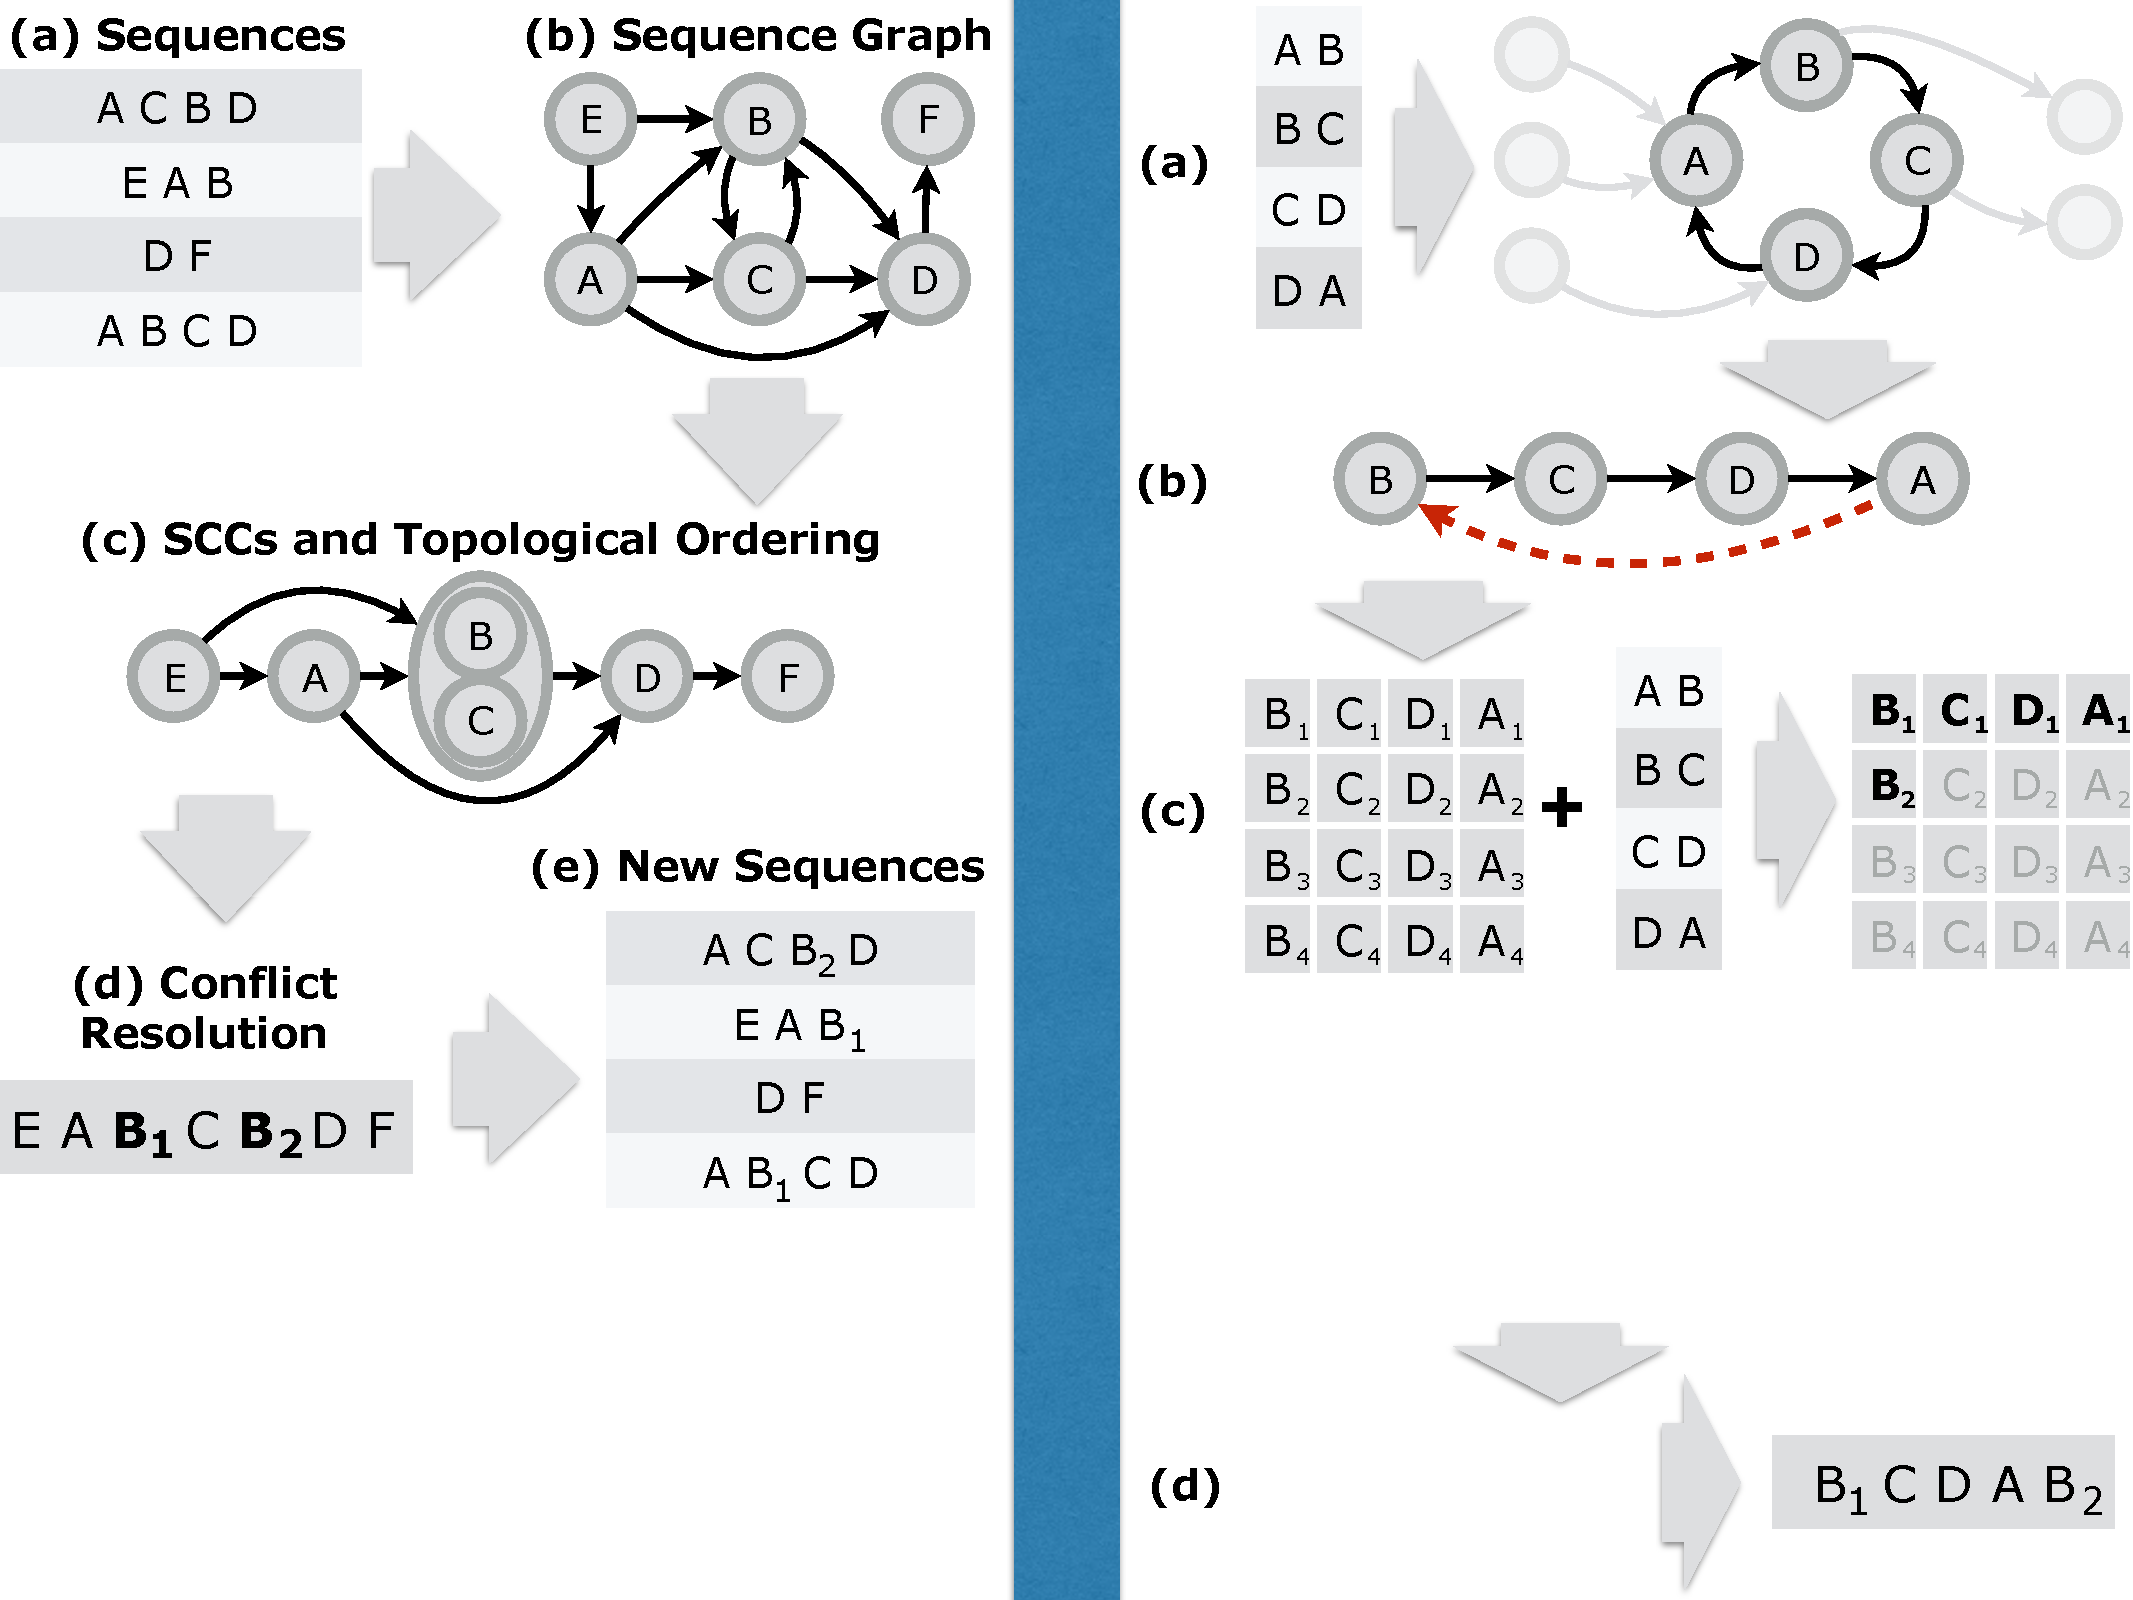
\includegraphics[trim={19.2cm 10cm 0 0}, clip, width=\linewidth]{figures/partial_ordering}
\end{subfigure} 
\end{minipage} 
\caption{This details the order-inconsistency resolution step of the algorithm. (a) shows a SCC of four attributes. (b) shows an 'almost' ordering of the SCC nodes, which minimizes the number of backward edges. (c) shows a  construction of a worst-case quadratically-sized universe, which is then traversed by every sequence to determine which attributes to splits for the new ordering.}
\label{fig:conflict_res}
\end{figure}
 


\section{Evaluation} \label{sec:evaluation}
SECTION NOT YET UPDATED. Not worth proofreading yet. 

We will now demonstrate the scalability of the supersets encoding scheme table size for a real exchange point. 

\subsection{Experimental Setup}
We used a data set from the AMS-IX exchange point~\cite{ams-ix}, which gave us access to 63 participants advertising over 600,000 prefixes. Although not on the scale of complete data sets of the largest exchange points, the data set is large enough that the partial masks optimization is required to fit masks into the MAC field. Our experiments were run on a laptop with a 4-core CPU running at 2.4GHz and 16GB of RAM.

The exchange point considered does not yet have support for SDN forwarding rules, so instead we simulate the number of forwarding entries required by the outbound policy of a hypothetical participant which is able to see all available route announcements. The participant was given 1000 uniformly random forwarding entries to a uniformly random subset of participants, with each subset size corresponding to a different experiment. 

\subsection{Performance}
We run our evaluations against a RIB dump of AMS-IX retrieved on May 1st, 2016 from the RIPE Routing Information Service raw data webpage~\cite{ris}.

\begin{figure}[t!] 
\begin{minipage}{1\linewidth}
\begin{subfigure}[b]{0.96\linewidth}
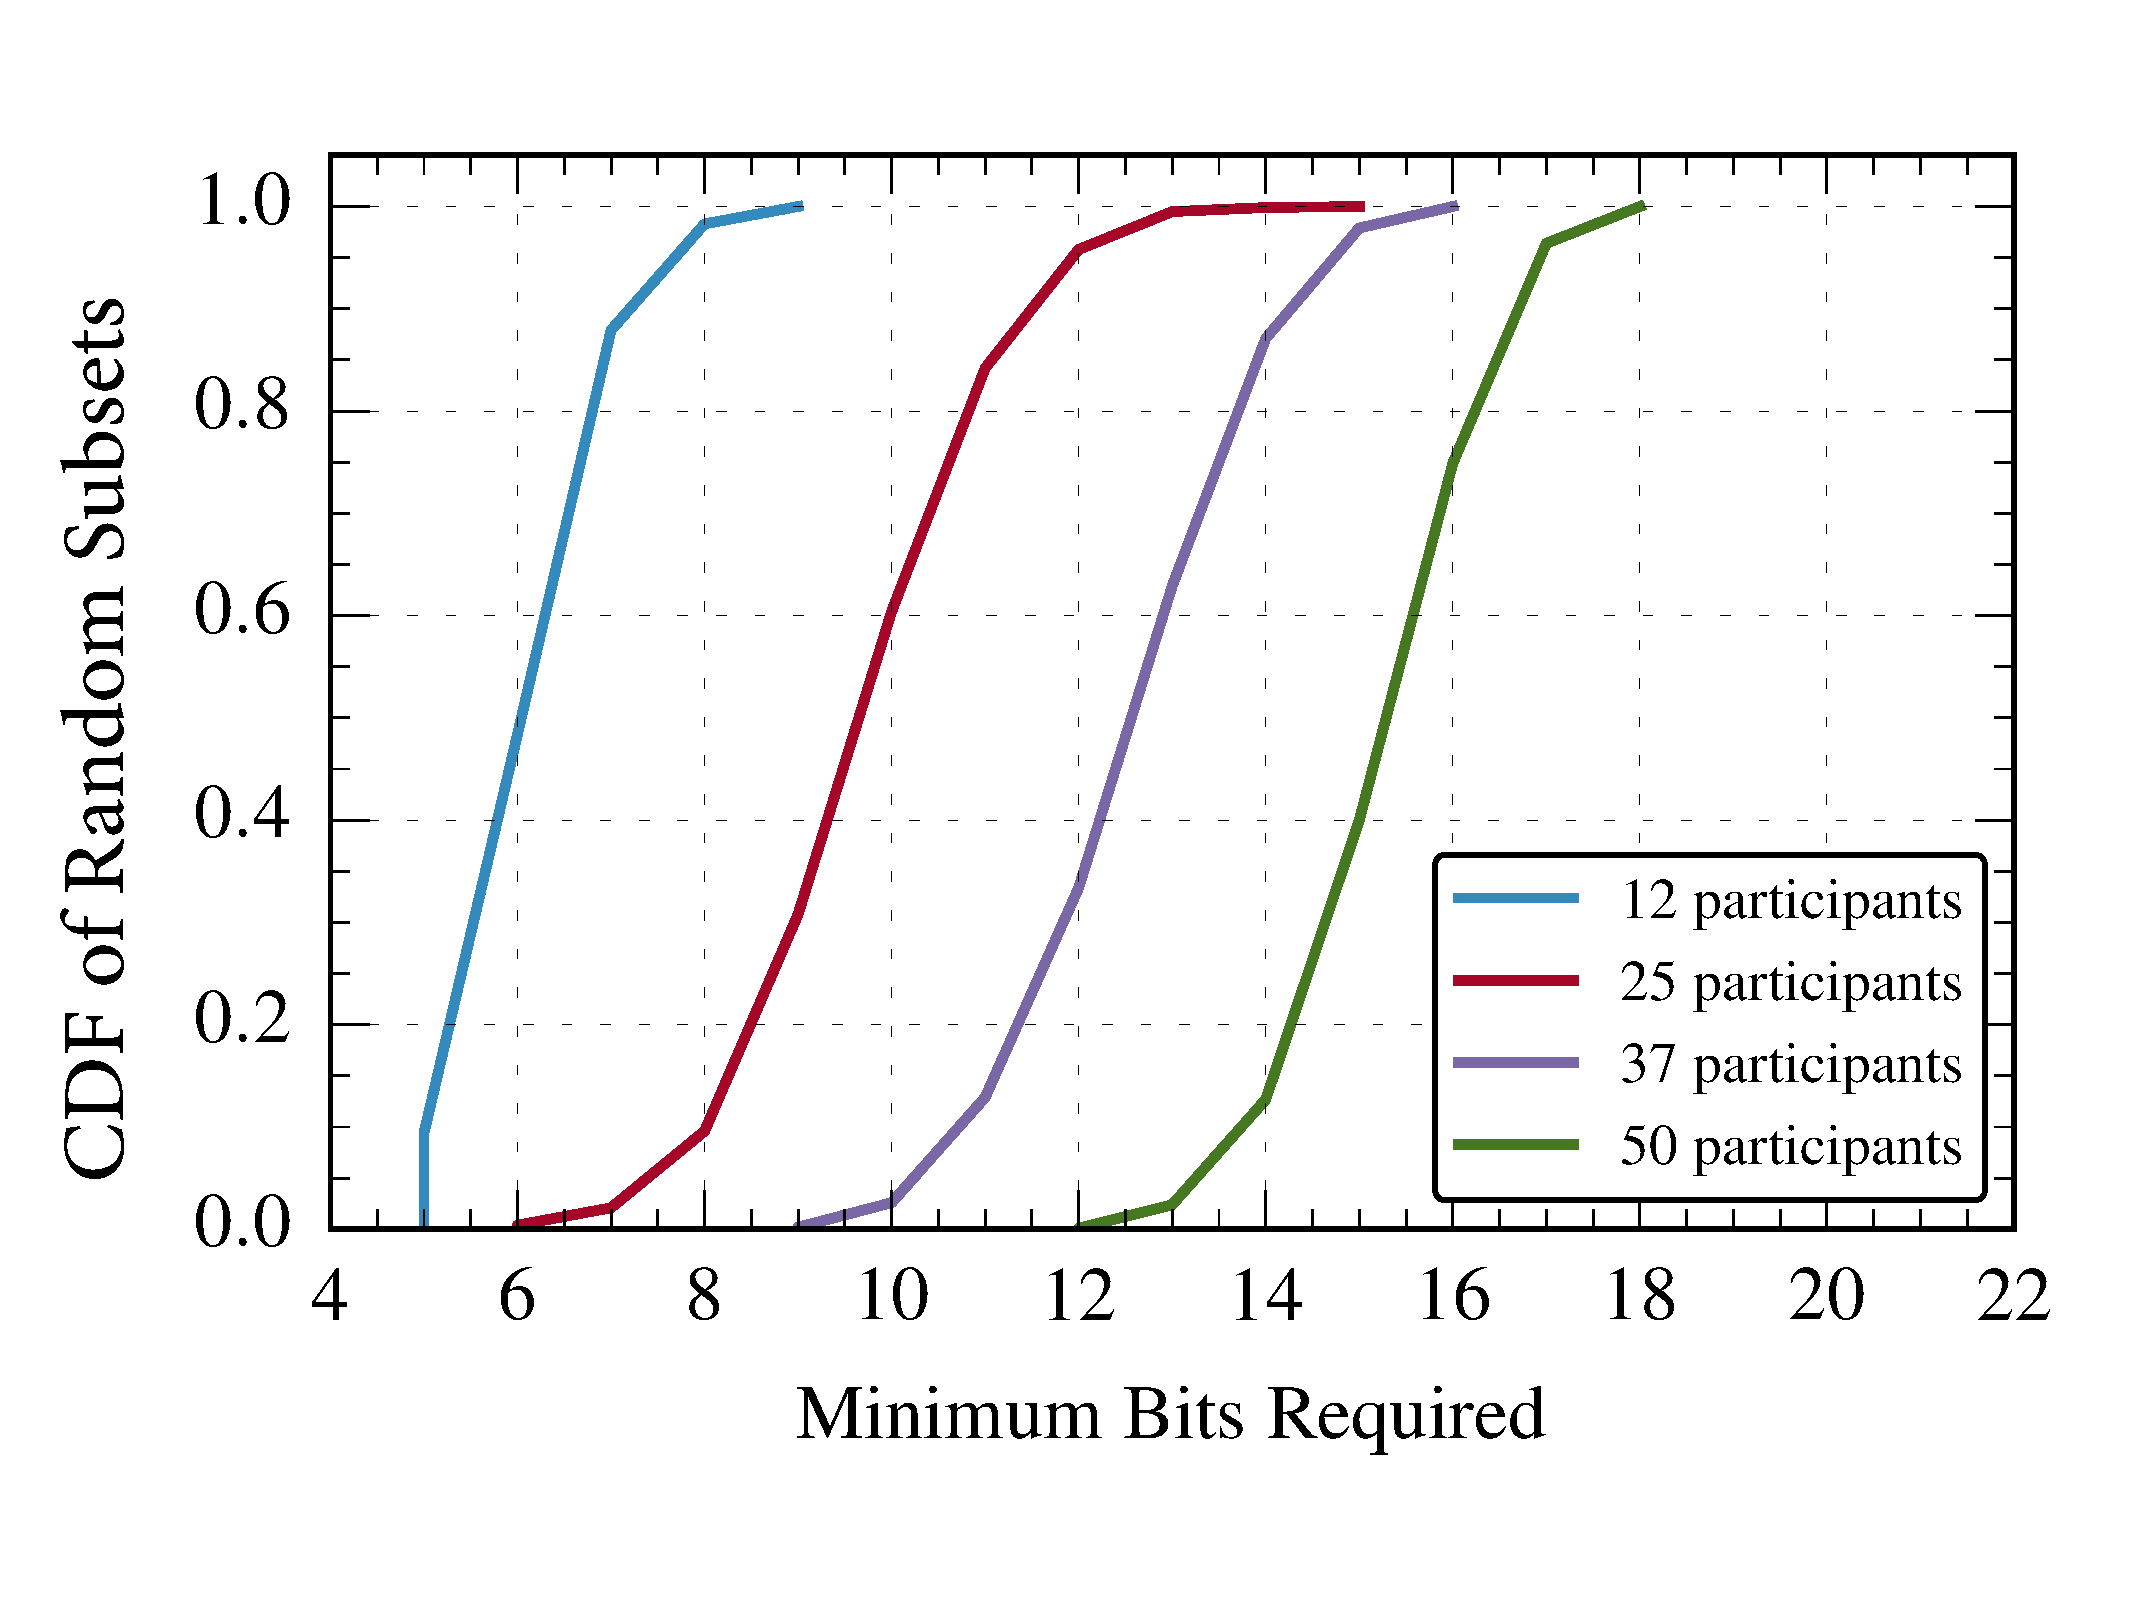
\includegraphics[width=\linewidth]{figures/bit_counts}
\end{subfigure} 
\end{minipage} 
\caption{Minimum number of bits required by a feasible solution for a random policy which forwards to a random subset of participants.}
\label{fig:bits}
\end{figure}

In order for our encoding scheme to successfully work, it must compress the information to the point that it fits into the MAC address field, which is restricted to 48 bits if no other information is encoded alongside reachability. Figure \ref{fig:bits} shows the number of bits required by our reachability encoding with uniformly randomly chosen active sets, repeated 500 times for each active set size. In the worst case, 18 bits were required when considering all 63 participants. The graphs appear to show that the number of bits required scales linearly with the number of participants present in the active set. However, we believe that the number of bits required actually scales sublinearly with the size of the active set, and that the appearance of linear scaling is a consequence of our simulation method. In order for the bits required to scale linearly, the number of participants that simultaneously advertise a single precept would have to also increase linearly in the size of the IXP, but we suspect this is not the case. Even if the number of bits required were indeed to scale linearly, extrapolating out the graph yields that, in the worst case, a participant's active set could contain over 100 participants, allowing very complex forwarding policies.

\begin{figure}[t!] 
\begin{minipage}{1\linewidth}
\begin{subfigure}[b]{0.96\linewidth}
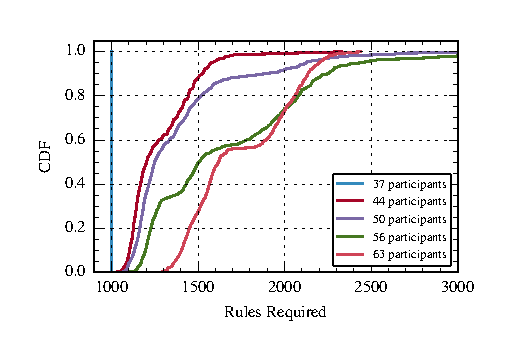
\includegraphics[width=\linewidth]{figures/rule_cdf}
\end{subfigure} 
\end{minipage} 
\caption{Number of rules required after encoding for a random policy of 1000 rules to random subsets of participants.}
\label{fig:rules}
\end{figure}

Figure \ref{fig:rules} shows the number of rules required by our encoding scheme after running the greedy algorithm with a bit limit of 37, allowing 11 bits for the ``mini-MAC". In this experiment, we began with a baseline policy of 1000 rules, with each rule forwarding to a participant chosen uniformly at random from a random active set. The experiment was repeated 500 times for each active set size, and the number of rules required after applying our encoding was plotted. When the active set is of size 37 or fewer, all participants can fit into a single mask, resulting in zero rule inflation. For active sets of size greater than 37, we can see that the inflation factor is at most 2 in the average case and 3 in the worst case for all active sets. 


\begin{figure}[t!] 
\begin{minipage}{1\linewidth}
\begin{subfigure}[b]{0.96\linewidth}
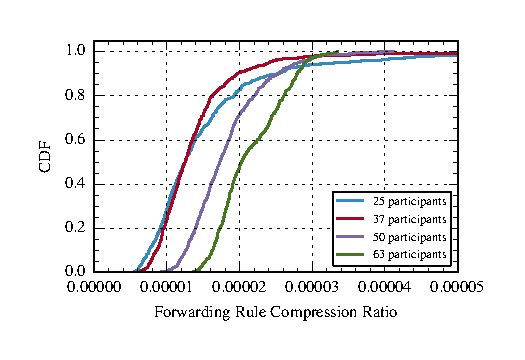
\includegraphics[width=\linewidth]{figures/compression_cdf}
\end{subfigure} 
\end{minipage} 
\caption{Ratio of flow rules required by our encoding algorithm versus the uncompressed
case on random policies involving random subsets of participants.}
\label{fig:compression}
\end{figure}

Figure \ref{fig:compression} shows how the number of flow rules generated by our approach compares to the naive case of zero compression. The compression ratio of our approach versus the naive approach is 20,000 to 1 in the worst case for all active set sizes, and 50,000 to 1 in the median case.


\begin{figure}[t!] 
\begin{minipage}{1\linewidth}
\begin{subfigure}[b]{0.96\linewidth}
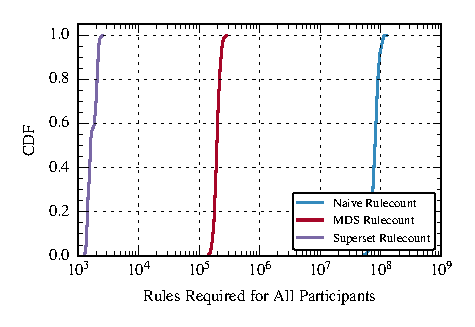
\includegraphics[width=\linewidth]{figures/comparison_cdf}
\end{subfigure} 
\end{minipage} 
\caption{Comparison of the number of flow rules required by our encoding algorithm to the previous state-of-the-art MDS encoding algorithm and the uncompressed case for a random policy involving all participants.}
\label{fig:comparison}
\end{figure}


Figure \ref{fig:comparison} compares our approach to the uncompressed case, as well as to the previous state-of-the-art, the MDS algorithm used in the original SDX system~\cite{gupta2014sdx}. The comparisons were made using the same approach of generating 1000 random rules, except for the MDS simulation. The MDS algorithm requires each prefix's default next-hop as part of the input, so in each trial we chose next-hops uniformly at random from the list of available next-hops. The graph shows that our approach consistently compresses the number of flow rules by two orders of mangitude greater than the MDS algorithm, which itself compressed the number of flow rules required by the naive case by three orders of magnitude. 

\begin{figure}[t!] 
\begin{minipage}{1\linewidth}
\begin{subfigure}[b]{\linewidth}
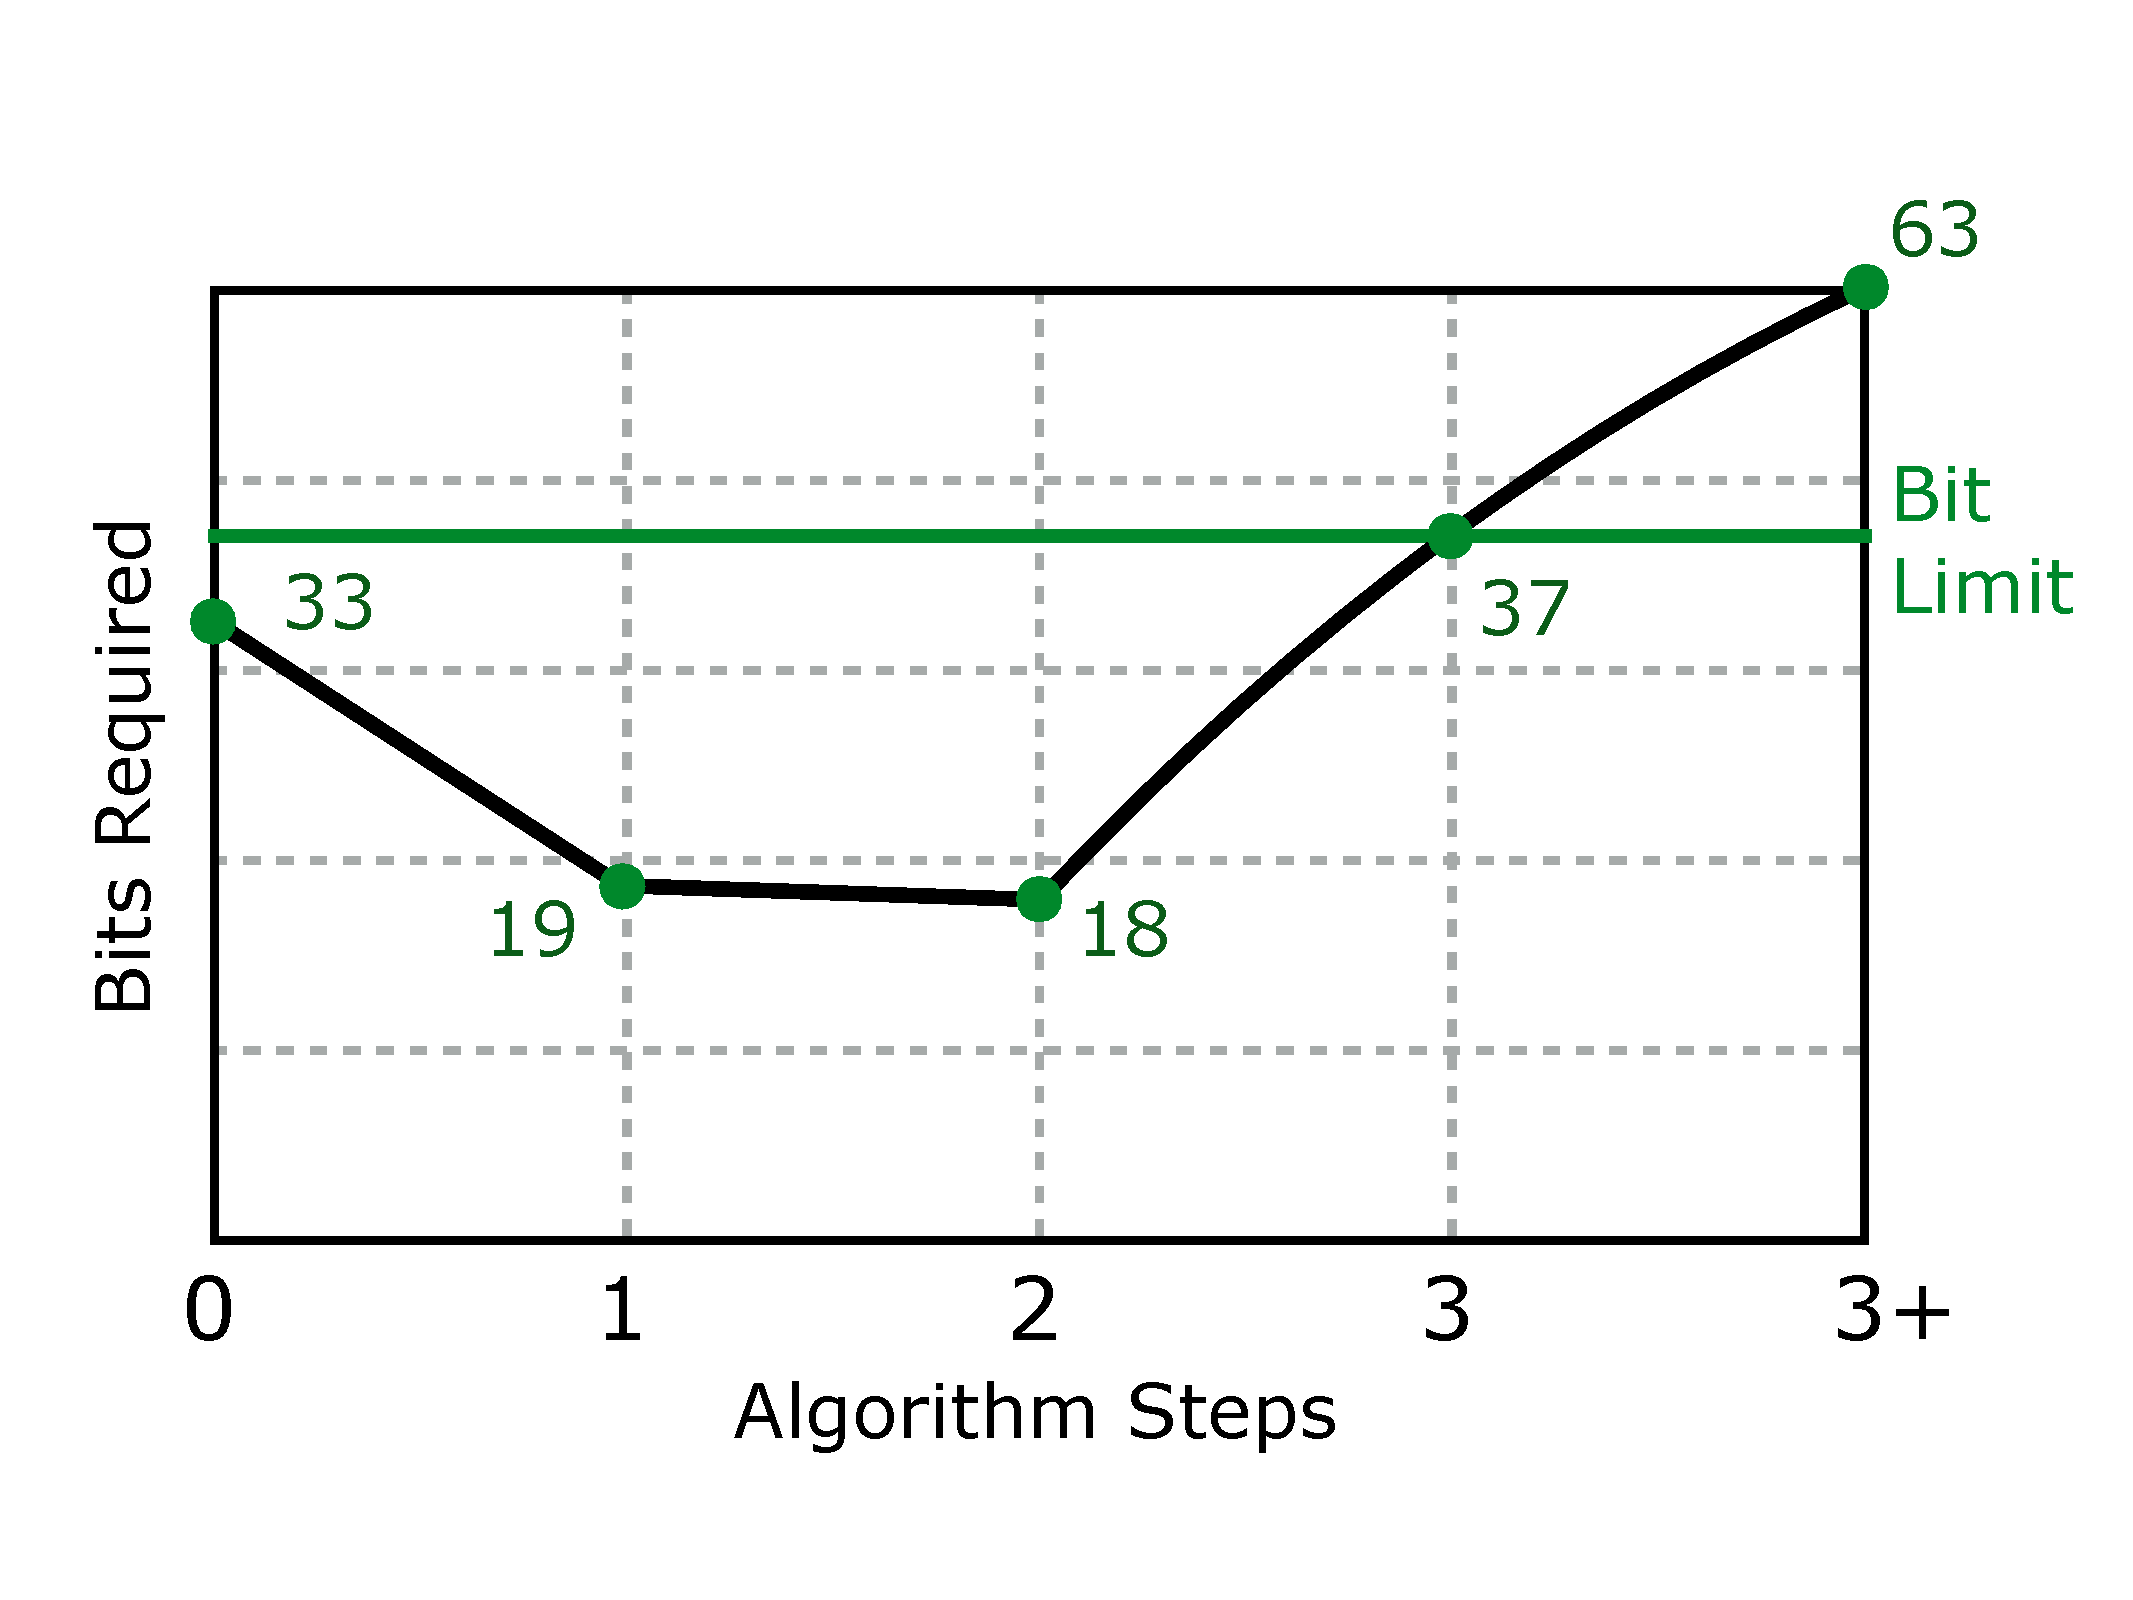
\includegraphics[width=\linewidth]{figures/bit_graph}
\end{subfigure} 
\end{minipage} 
\caption{Graph of the number of bits required by the encoding scheme at each step of the algorithm, shown with real values computed over the AMS-IX RIPE data set. Step 0 is the input of all sets, step 1 is removal of subsets, step 2 is attempting greedy bit minimization, step 3 is after greedily decreasing inflation up to the bit limit, and step 3+ is with no bit limit. }
\label{fig:bit_graph}
\end{figure}
\section{Related Work} \label{sec:related}

Variable-length prefix codes have been used for various applications. In the seminal work of Huffman~\cite{Huffman} an algorithm for an optimal selection of them was described for lossless compression of a source symbol. The selection minimizes the encoding length by using fewer bits for common symbols, achieving results close to lower bounds from information theory. More recently, they were suggested to encode paths as a sequence of nodes while focusing one reducing the maximum length of any encoded path~\cite{PathEncoding}. A similar approach was suggested for the encoding for fixed-width memories~\cite{FixedMemories}. In all these schemes, the encoding is given by the concatenating the codes of the attributes, thus is often long for a large number of possible attributes. On the contrary, in the suggested scheme the dependency is only in the number of unique groups and the number of attributes in a set.


Alpaca~\cite{alpaca} also aims to embed attributes of each flow into the packet header with the goal of easing network policy enforcement, but does not follow the FEC tagging abstraction. Instead, they embed attributes into the hosts' IP address assignments, which adds the constraint that attribute encodings must be unique for each host. 

Flowtags~\cite{flowtags} uses flat tagging to associate each packet with a source host and a middlebox path, even in the face of middleboxes which modify packet headers. Their approach relies upon modifications of the source code of each middlebox to be able to read and write the tags. Our approach allows middleboxes to be unaware of tags, but at the cost of having no source host association which is readable by middleboxes. Tags are attached to packets by the first middlebox that the packets traverse. This implies that the packets must be steered to the first middlebox by some other means. Rules for decoding the tags are installed reactively as network nodes see tags for the first time. 

The SDX~\cite{sdx} project uses flat tagging to attach to packets a list of valid next-hops that packets can take through an internet exchange point . This list is then used to correctly enforce interdomain SDN policies that exchange point members install themselves. Tags are attached to packets by controller responses to ARP requests with tags as the destination MAC addresses. Rules for decoding the tags are installed proactively in the exchange point fabric.

SDX was followed by the iSDX~\cite{isdx} project, which aimed to address some of the scalability challenges that the first project faced. Namely, the number of rules needed to decode tags was prohibitively large in SDX, preventing any reasonably-sized IXP from implementing the project on commodity switches. One of the key changes that the iSDX project made to improve scalability was the introduction of a new tagging scheme which utilized wildcard matching. This tagging scheme is the precursor to our work. The tag attachment and decoding model mimicked the first SDX.

Bloom filter~\cite{Bloom} is a popular data structure for set representation. It supports membership queries and relies on a bit array. Bloom filter suffers from an inherent false positive error, where some elements can be wrongly reported as members of the set. While minimizing the tag width is an key property of our scheme, the Bloom filter memory is several times larger than the number of elements, e.g. 10-20 times for a false positive probability of 0.01\% - 1\%. Moreover, Bloom filter relies on hashing which might not be available in some switch architectures.


\input{Conclusion}

%\end{sloppypar}

%\vspace{-0.01in}
%\section*{Acknowledgments}
% Comments for people we need to acknowledge in the final version.
\noindent \textbf{Acknowledgments.}
Fill me in
%\pagebreak
%\small
%\setlength{\bibsep}{0pt}
%\setlength{\parskip}{-1pt}
%\setlength{\itemsep}{-1pt}
% \footnotesize % SPACE
\balance
\bibliography{paper}
\bibliographystyle{acm}
%\bibliographystyle{abbrvnat_noaddr} % SPACE
%\theendnotes % ENDNOTES
}{% onlyAbstract
}

%\pagebreak
%\input{appendix}

\end{document}

%%%%%%%%%%%%%%%%%%%%  END OF DOCUMENT  %%%%%%%%%%%%%%%%%%%%
